\documentclass[12pt, a4paper]{article}
\usepackage{enumitem} % Brukes til enumerering med bokstaver.
\usepackage{amssymb} % Symboler som kompliment etc.
\usepackage{amsmath}
\usepackage{venndiagram}
\usepackage{tikz} 
\usetikzlibrary{patterns}

\title{Oblig 2.}
\author{Joakim Johannesen}
\date{2023}

\begin{document}
\maketitle

 \section*{2.1.4}
 \addcontentsline{toc}{section}{2.1.4}
   $A \subseteq B$ og $B \subseteq C$

 \section*{2.1.5}
 \addcontentsline{toc}{section}{2.1.5}
   a. ettersom $ 4\in A$.\\
   c. ettersom $ 0\notin A$.\\
   e. ettersom $ \{1\} \subseteq A$.\\
   i. ettersom $ \{1,3,4\} \subseteq A$.
   
 \section*{2.2.1}
 \addcontentsline{toc}{section}{2.2.1}
   \begin{enumerate} [label=\alph*.]
      \item $ A \cup B = \{1,2,3,4,5\} $
      \item $ A \cap B = \{3,4\} $
      \item $ A - B = \{1,2\} $
      \item $ B - A = \{5\} $
   \end{enumerate}

\newpage 

 \section*{2.2.2}
 \addcontentsline{toc}{section}{2.2.2}
   \begin{enumerate} [label=\alph*.]
      \item $ (A\cup B)\cap C = \{1,2\} $
      \item $ A\cup (B\cap C) = \{1,2,3,4\} $
      \item $ {\overline{A}} \cap C = \{7\} $
      \item $ {\overline{(A\cup C)}} \cap B = \{5\} $
      \item $ (A\cup B) - C = \{3,4,5\} $
      \item $ \overline{C} = \{3,4,5,6,8\} ,\quad \overline{A} = \{5,6,7,8\}\\
      (\overline{C}-B) = \{6,8\}\\
      (\overline{C}-B) - \overline{A} = \emptyset $
   \end{enumerate}
\section*{2.3.1}
  \addcontentsline{toc}{section}{2.3.1}
   $ A \times B = \{(1,a), (1,b), (2,a), (2,b), (3,a), (3,b)\} $

\newpage

\section*{Oppgave 1.}
\addcontentsline{toc}{section}{Oppgave 1.}
   $ A = B = C = D $
\section*{Oppgave 2.}
\addcontentsline{toc}{section}{Oppgave 2.}
   \begin{enumerate} [label=\alph*.]
      \item $ A = \{1, 3, 5, 7, 9\} $
      \item $ B = \{-2, -1, 0, 1, 2\} $
      \item $ C = \{0,2,0,2,\dots\} $
      \item $ D = \{\dots ,-3,-2,-1,0,7,8,9,\dots\} $
   \end{enumerate}

\section*{Oppgave 3.}
\addcontentsline{toc}{section}{Oppgave 3.}
   \begin{enumerate} [label=\alph*.]
      \item $ A \cup \emptyset = \{0\} $
      \item $ A \cup B = \{0,1,2,3\} $
      \item $ \lvert A \rvert = 1 $
      \item $ \lvert B \rvert = 3 $
      \item $ \lvert A \cup B \rvert = 4 $
      \item $ \overline{B\cap C} = \{0,1,4,5,6,7,8,9\} $
      \item $ P(C) = \{\emptyset,\{2\},\{3\},\{5\},\{2,3\},\{2,5\},\{2,3,5\}\} $
      \item $ B \times C = \{(1,2), (1,3), (1,5), (2,3), (2,5), (3,2), (3,3), (3,5)\} $
   \end{enumerate}

\newpage

\section*{Oppgave 4.}
\addcontentsline{toc}{section}{Oppgave 4.}
   a og b er ekvivalente. Samt er d og e.\\
   \begin{enumerate} [label=\alph*.]
      \item \begin{venndiagram3sets} \fillBCapCNotA \fillOnlyB \end{venndiagram3sets}
      \item \begin{venndiagram3sets} \fillBCapCNotA \fillOnlyB \end{venndiagram3sets}
      \item \begin{venndiagram3sets} \fillOnlyA \fillOnlyB \fillACapBNotC \end{venndiagram3sets}
      \item \begin{venndiagram3sets} \fillOnlyA \end{venndiagram3sets}
      \item \begin{venndiagram3sets} \fillOnlyA \end{venndiagram3sets}
      \item \begin{venndiagram3sets} \fillOnlyC \end{venndiagram3sets}
   \end{enumerate}

\section*{Oppgave 5.}
\addcontentsline{toc}{section}{Oppgave 5.}
   \begin{enumerate} [label=\alph*.]
      \item 
         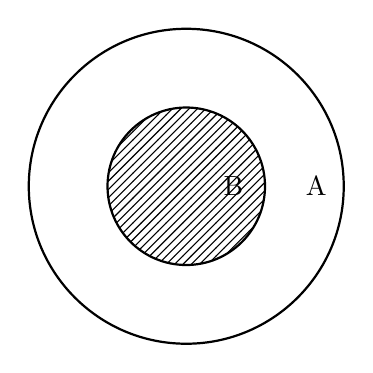
\begin{tikzpicture}
           % Sirkelen A
           \draw[thick] (0, 0) circle (2cm);
           \fill[pattern={north east lines}] (0, 0) circle (1cm);
           \node at (1.65, 0) {A};
           
           % Sirkelen B
           \draw[thick] (0, 0) circle (1cm);
           \node at (0.6, 0) {B};
           
         \end{tikzpicture}
      \item 
         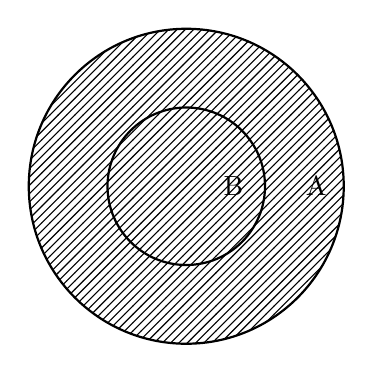
\begin{tikzpicture}
           % Sirkelen A
           \draw[thick] (0, 0) circle (2cm);
           \fill[pattern={north east lines}] (0, 0) circle (2cm);
           \node at (1.65, 0) {A};
           
           % Sirkelen B
           \draw[thick] (0, 0) circle (1cm);
           \node at (0.6, 0) {B};
           
         \end{tikzpicture}
      \item 
         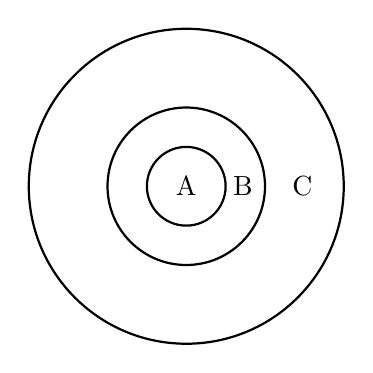
\begin{tikzpicture}
           % Sirkelen A
           \draw[thick] (0, 0) circle (2cm);
           \node at (1.475, 0) {C};
           
           % Sirkelen B
           \draw[thick] (0, 0) circle (1cm);
           \node at (0.72, 0) {B};

           % Sirkelen C
           \draw[thick] (0, 0) circle (0.5cm);
           \node at (0,0) {A};
         \end{tikzpicture}

   \end{enumerate}

\section*{Oppgave 6.}
\addcontentsline{toc}{section}{Oppgave 6.}
   $ A \cap (B - A) \quad \text{Vi husker ekvivalensen fra oppgave 4.} \\
   = A \cap (\overline{A} \cap B) \quad \text{Assosiative loven.} \\
   = (A \cap \overline{A}) \cap B \quad \text{Inversloven.} \\
   = \emptyset \cap B \quad \text{Dominansloven.} \\
   = \emptyset $ \\
   Vi sitter dermed igjen med den tomme-mengde.
\end{document}